\documentclass{article}
\usepackage{graphicx} % Required for inserting images
\usepackage{float}
\usepackage[T1]{fontenc}
\usepackage{amsmath}
\usepackage[margin=1in]{geometry}
\usepackage{booktabs}
\usepackage{tabularx}
\usepackage[hidelinks]{hyperref}

\title{Leaving high-VRP puts unhedged on the stress-sized SPY put book}
\author{Experiment report \textperiodcentered{} L/S Gamma Desk, QUANTT}
\date{2026-11-02}

\begin{document}

\maketitle

\textbf{Question:} On the 35\% stress-sized \texttt{hedged} put book, does leaving a new put unhedged for its whole life when VRP at entry is above 2 vol points earn more than always hedging, with a better Sharpe ratio?

\textbf{Method:}

\begin{itemize}

\item \textbf{Pre-registration.} The hypothesis card was committed before any run (commit 954824c).

\item \textbf{Data and book.} The 2026-10-22 \texttt{hedged} book is replayed on R2 replay snapshots v1 (config\_hash b040760187f0) over the development window 2014-06-02 to 2024-12-31. The hold-out (2025-01-01 to 2026-07-10) was not used.

\begin{itemize}

\item The book is an always-on short 25-delta put, sized at entry to a 35\% stress budget: a one-day 20\% drop with IV at max(60\%, the put's IV) may cost at most \$87,500.

\item It is hedged daily at 10:15 with a 10-share band.

\end{itemize}

\item \textbf{New switch.} Research-only \texttt{[backtest] vrp\_\allowbreak{}unhedge}. A put entered when VRP (ATM IV minus the GARCH forecast, at the 10:15 decision) is above the cutoff is never hedged. It is sized to the unhedged stress loss, so it stays within the 35\% budget.

\item \textbf{Variants:} \texttt{vrp2} = cutoff 0.02, the live short band (primary); \texttt{vrp1} = 0.01; \texttt{vrp4} = 0.04.

\item \textbf{Reference.} The registered \texttt{2026-\allowbreak{}10-\allowbreak{}22-\allowbreak{}stress-\allowbreak{}sized-\allowbreak{}puts/\allowbreak{}hedged} runs, reused and not rerun, at the same spread multiple. The registered 2026-10-22 \texttt{unhedged} book is shown for context.

\item \textbf{Runs and costs.} Every variant was run at 1x and 2x spreads. Costs are \$0.65 per contract and \$0.005 per share, with a \$1 minimum per order. Exits and hedges run at 10:15 ET.

\end{itemize}

This report was written by Claude at the PM's request.

\section{Result vs the pass bar}

Every check had to hold at 1x and 2x. P\&L is net of spreads and commissions, in USD, for the sized book.

\begin{center}\small
\begin{tabularx}{\linewidth}{>{\raggedright\arraybackslash}X l l l l l}
\toprule
\textbf{Check (\texttt{vrp2} vs \texttt{hedged})} & \textbf{1x value} & \textbf{1x bar} & \textbf{2x value} & \textbf{2x bar} & \textbf{Result} \\
\midrule
Net P\&L, full window & \$114,100 & > \$121,482 & \$87,924 & > \$101,172 & fail \\
Net P\&L, 2014-06 to 2019-12 & \$54,493 & > \$49,132 & \$44,526 & > \$42,687 & pass \\
Net P\&L, 2020-01 to 2024-12 & \$59,608 & > \$72,350 & \$43,398 & > \$58,485 & fail \\
Sharpe ratio, full window & 0.51 & > 0.52 & 0.39 & > 0.43 & fail \\
Max drawdown & \$73,622 & \ensuremath{\leq} \$87,500 & \$78,839 & \ensuremath{\leq} \$87,500 & pass \\
Unhedged round trips (floor \ensuremath{\geq} 20, 1x) & 45 &  &  &  & met \\
\bottomrule
\end{tabularx}
\end{center}

\textbf{Verdict: failed.} Leaving high-VRP puts unhedged made \$7.4k less than always hedging at 1x and \$13.2k less at 2x, at a slightly lower Sharpe. The book still makes money: +\$114k at 1x and +\$88k at 2x.

\subsection{Full-window numbers (not part of the bar)}

\textbf{1x spreads}

\begin{center}\small
\begin{tabularx}{\linewidth}{>{\raggedright\arraybackslash}X >{\raggedright\arraybackslash}X >{\raggedright\arraybackslash}X >{\raggedright\arraybackslash}X >{\raggedright\arraybackslash}X >{\raggedright\arraybackslash}X}
\toprule
\textbf{} & \textbf{hedged} & \textbf{unhedged (2026-10-22)} & \textbf{vrp2} & \textbf{vrp1} & \textbf{vrp4} \\
\midrule
Net P\&L & \$121,482 & \$253,839 & \$114,100 & \$149,178 & \$141,397 \\
Sharpe & 0.52 & 0.80 & 0.51 & 0.65 & 0.57 \\
Max drawdown & \$70,362 & \$58,469 & \$73,622 & \$73,622 & \$66,174 \\
ES 5\% (daily) & \ensuremath{-}\$3,016 & \ensuremath{-}\$5,195 & \ensuremath{-}\$3,373 & \ensuremath{-}\$3,449 & \ensuremath{-}\$3,245 \\
Round trips & 182 & 412 & 208 & 218 & 196 \\
Option /\allowbreak{} hedge commissions & \$5,955 /\allowbreak{} \$2,868 & \$9,300 /\allowbreak{} \$0 & \$6,300 /\allowbreak{} \$2,671 & \$6,506 /\allowbreak{} \$2,603 & \$6,199 /\allowbreak{} \$2,764 \\
\bottomrule
\end{tabularx}
\end{center}

\textbf{2x spreads}

\begin{center}\small
\begin{tabularx}{\linewidth}{l l >{\raggedright\arraybackslash}X l l l}
\toprule
\textbf{} & \textbf{hedged} & \textbf{unhedged (2026-10-22)} & \textbf{vrp2} & \textbf{vrp1} & \textbf{vrp4} \\
\midrule
Net P\&L & \$101,172 & \$239,831 & \$87,924 & \$146,791 & \$120,623 \\
Sharpe & 0.43 & 0.75 & 0.39 & 0.64 & 0.48 \\
Max drawdown & \$75,488 & \$59,859 & \$78,839 & \$75,413 & \$72,197 \\
\bottomrule
\end{tabularx}
\end{center}

\section{Charts}

\begin{figure}[H]\centering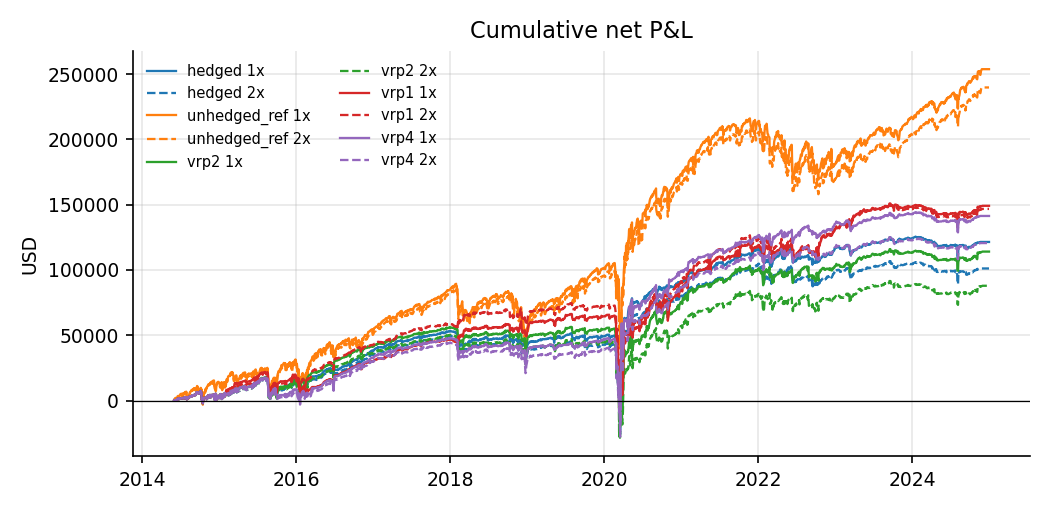
\includegraphics[width=0.92\linewidth]{figures/cum_pnl.png}\caption{Cumulative net P\&L, 1x solid and 2x dashed}\end{figure}

\texttt{vrp2} and \texttt{vrp4} track the hedged book until February 2020; \texttt{vrp1} is about \$15k ahead by the end of 2019. In March 2020 \texttt{vrp2} and \texttt{vrp1} fall further and recover less than \texttt{hedged}. \texttt{vrp4} comes out of March 2020 ahead. After 2020 all three run roughly parallel to \texttt{hedged}, far below the always-unhedged book.

\begin{figure}[H]\centering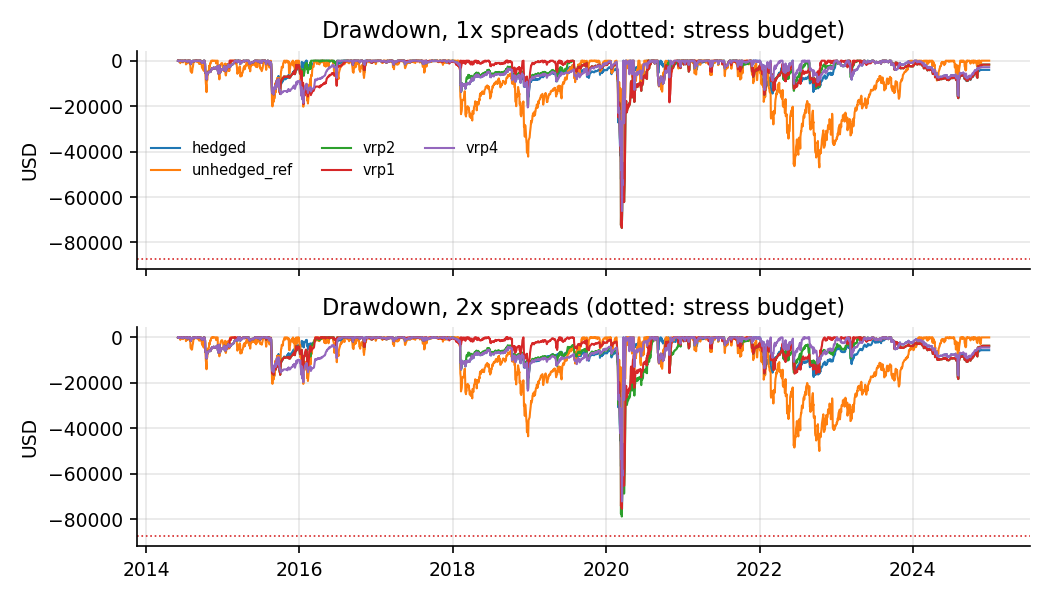
\includegraphics[width=0.92\linewidth]{figures/drawdown.png}\caption{Drawdown at 1x and 2x spreads}\end{figure}

Every book's worst drawdown is in March 2020, and all stay inside the \$87,500 budget. \texttt{vrp2}'s is the deepest of the hedged-type books at 2x, at \$78.8k.

\begin{figure}[H]\centering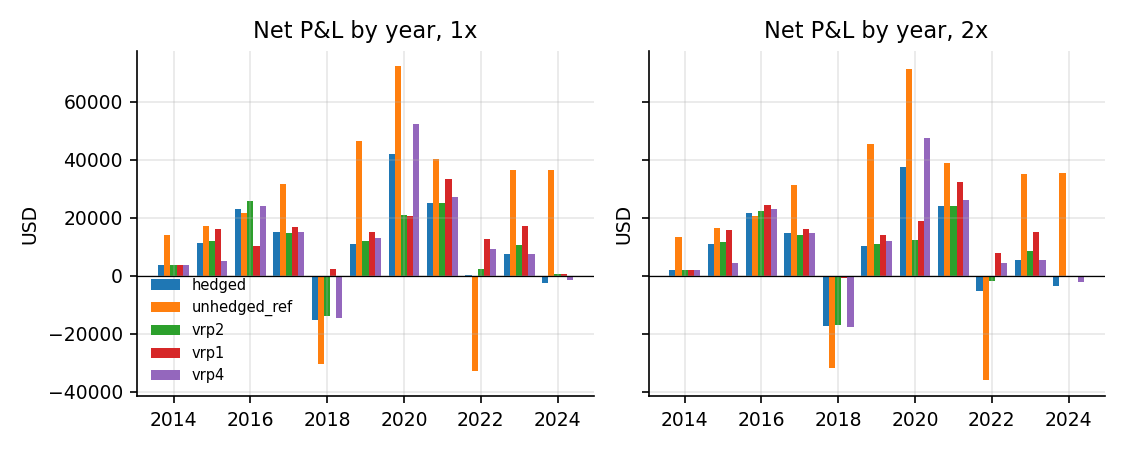
\includegraphics[width=0.92\linewidth]{figures/yearly.png}\caption{Net P\&L by year}\end{figure}

At 1x, \texttt{vrp2} is within about \$3.4k of \texttt{hedged} in every year except 2020, where it made \$21.1k less. The always-unhedged book is far ahead in most years, but it lost \$30k in 2018 and \$33k in 2022.

\begin{figure}[H]\centering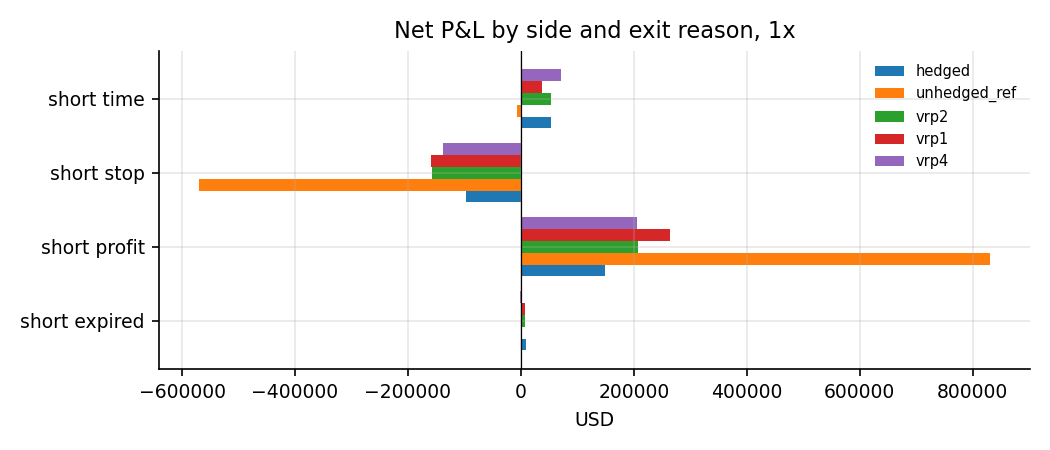
\includegraphics[width=0.92\linewidth]{figures/by_reason.png}\caption{Net P\&L by side and exit reason, 1x}\end{figure}

The VRP variants take larger stop losses and larger profit-takes than \texttt{hedged}, because their unhedged puts swing with SPY. The always-unhedged book shows the same pattern, much bigger.

\begin{figure}[H]\centering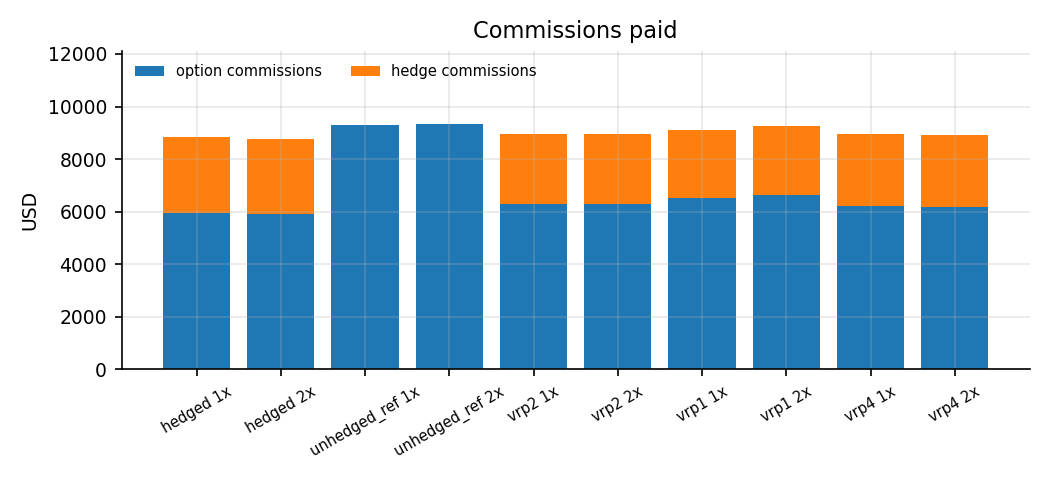
\includegraphics[width=0.92\linewidth]{figures/fees.png}\caption{Commissions paid}\end{figure}

Commissions barely change. Unhedged puts save some hedge orders, but the variants open more positions, so option commissions rise slightly.

\begin{figure}[H]\centering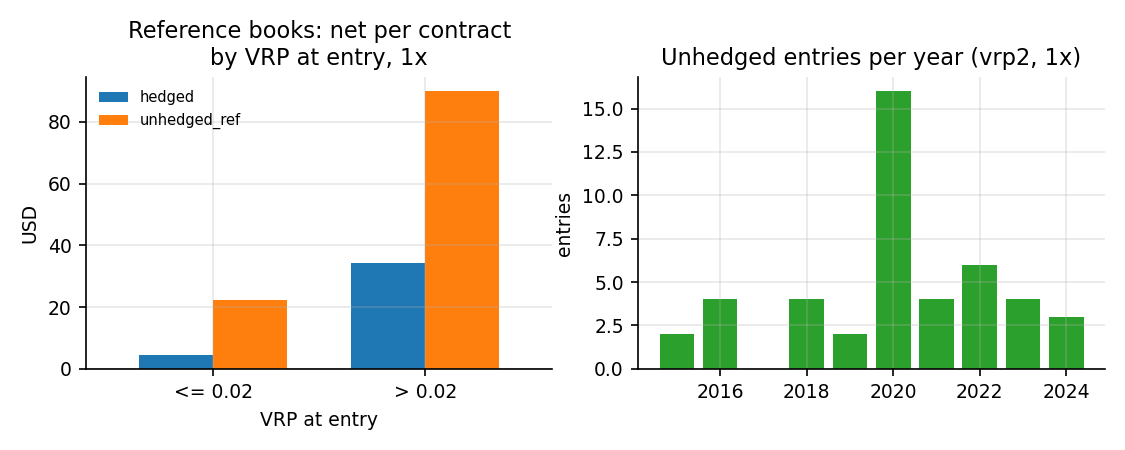
\includegraphics[width=0.92\linewidth]{figures/vrp_split.png}\caption{Reference books' net per contract by VRP at entry, and vrp2's unhedged entries per year}\end{figure}

\textbf{Left:} in both reference books, puts entered with VRP above 2 points earned more per contract on average (the mean of each round trip's net per contract). The always-unhedged book made \$90 per contract on them, against \$22 on the rest. Pooled (total net over total contracts), the unhedged book's split is \$80 against \$27, but the hedged book's reverses: \$20.6 against \$25.5.

\textbf{Right:} \texttt{vrp2} went unhedged on 45 entries. Sixteen of them were in 2020, the year it lost ground.

\section{Analysis}

\textbf{The VRP timing idea works in its delta leg.} The question is whether a high VRP predicts that the put's equity exposure will pay. For the always-unhedged 2026-10-22 book, I split the P\&L of holding the put's delta in SPY between 10:15 decisions by VRP at entry:

\begin{itemize}

\item \textbf{VRP above 2 points:} delta earned 64\% a year per dollar of delta held, over 248 position-days.

\item \textbf{Puts entered at or below 2 points:} 9.5\% a year, over 2,217 position-days.

\item The high-VRP delta P\&L was positive in every one of the ten years with such entries. Excluding 19 February to 30 April 2020 it is 73\% a year.

\end{itemize}

In \texttt{vrp2} itself, the 45 unhedged puts earned \$56.9k of delta P\&L over 247 position-days, 46\% a year per dollar of delta. On its own position mix, \texttt{vrp2} is doing what the hypothesis says. Within \texttt{vrp2}, the 45 unhedged round trips made \$36.2k, on average \$54 per contract per round trip. The 163 hedged ones made \$74.1k, on average \$7.8 per contract (pooled: \$46.1 against \$18.1).

\textbf{Two things cost more than the timing gained.}

\begin{enumerate}

\item \textbf{Smaller size.} An unhedged put gets no hedge credit in the stress test, so it is sized smaller: 17.5 contracts on average, against 25.2 for \texttt{vrp2}'s hedged puts. Less premium is collected exactly when the premium is highest.

\item \textbf{One path change in March 2020.} The cost is concentrated there:

\begin{itemize}

\item On 2 March 2020 VRP was 3.4 points, so \texttt{vrp2} and \texttt{vrp1} opened that put unhedged; \texttt{hedged} opened it hedged.

\item The unhedged put hit its stop on 9 March, three trading days before the hedged book's put. The book re-entered on 10 March and held a new put into the 16-23 March crash.

\item It therefore missed the 100-contract entry on 13 March that made the hedged book \$70.7k.

\item From 19 February to 30 April 2020, \texttt{vrp2} lost \$7.6k while \texttt{hedged} made \$21.7k: a \$29.2k swing.

\item Outside that window, \texttt{vrp2} beat \texttt{hedged} by \$21.8k (\$121.7k against \$99.8k).

\item \texttt{vrp4}'s cutoff was above the 2 March VRP, so it kept the hedged book's March sequence. That is why it finished 2020 \$10.5k ahead of \texttt{hedged}, while \texttt{vrp2} and \texttt{vrp1} each finished about \$21k behind.

\end{itemize}

\end{enumerate}

\textbf{The result depends on the cutoff, and that is mostly path dependence.} Only 117 of \texttt{vrp2}'s 208 round trips open at the same time as one of the hedged book's, so one changed stop reshapes everything after it. \texttt{vrp1} beat \texttt{hedged} on every check at both spreads:

\begin{itemize}

\item net P\&L: +\$149.2k against \$121.5k at 1x, and +\$146.8k against \$101.2k at 2x;

\item Sharpe: 0.65 and 0.64, against 0.52 and 0.43.

\end{itemize}

But it is a pre-registered sensitivity, so promoting it would mean choosing the cutoff after seeing results, and it went through the same March 2020 change as \texttt{vrp2}. Its edge comes from elsewhere, mostly 2018 (+\$17.6k) and 2022 (+\$12.4k). \texttt{vrp4} beat \texttt{hedged} overall but failed 2014-2019.

The spread of results across cutoffs (\ensuremath{-}\$7k to +\$28k at 1x) is as large as any effect, so the sample can't pin down a cutoff.

\section{Verdict}

\textbf{Failed} on the pre-registered bar: the primary made less than always hedging at both spreads, with a slightly lower Sharpe. The evidence that high VRP predicts the put's delta return is encouraging but in-sample. The sizing rule gives that delta back, and one March 2020 path change outweighed it.

A follow-up would need its own card, for example:

\begin{itemize}

\item size unhedged high-VRP puts so the book's delta stays the same and only the hedge changes;

\item or test VRP as a hedge ratio (for example half-hedged) rather than an all-or-nothing switch.

\end{itemize}

\texttt{vrp1} should not be promoted from this card.

\section{Caveats}

\begin{itemize}

\item \textbf{In-sample.} The idea came from the 2026-10-22 results and the 2026-10-31 strategy report. Before pre-registration I saw the always-unhedged book's P\&L per contract split at 2 VRP points (the left panel above). Only the hold-out can confirm anything.

\item \textbf{Concentration.} The primary's shortfall comes from one sequence of trades in March 2020. Outside that window it is ahead.

\item \textbf{Spread model.} Fitted on about two weeks of calm 2026 live quotes; the 2x run is the stress test. Fills of 20-100 contracts use the same spread model as one contract.

\item \textbf{Margin.} Not modelled. An unhedged put needs less Reg-T margin than a put plus its short-share hedge. The hedged positions keep the margin problem noted in the 2026-10-22 report.

\item \textbf{Data gaps.} About 3.3\% of scheduled times are skipped because R2 has no snapshot.

\item \textbf{Few events.} 45 unhedged round trips for \texttt{vrp2} (floor 20), 58 for \texttt{vrp1} and 24 for \texttt{vrp4}.

\item \textbf{Delta split method.} The delta P\&L uses the snapshot delta at each 10:15 decision and the spot change to the next decision. It ignores gamma and vega, so it is an attribution, not a hedged return.

\end{itemize}

\section{Trials}

6 trials for this experiment: 3 variants at 1x and 2x, from one run of \texttt{experiment.\allowbreak{}py} at 954824c. The \texttt{vrp4} rows are tagged \texttt{954824c-\allowbreak{}dirty}: three other experiments of the same batch were running in the same working tree and had written figure files, and one had edited its own script. No engine, config or file of this experiment had changed. The registry holds 98 trials in all.

The reference was reused, not rerun, and the baseline's 2 trials are unchanged. After the run, the commissions chart's labels were fixed in \texttt{experiment.\allowbreak{}py} and the figures rebuilt with \texttt{-\allowbreak{}-\allowbreak{}report-\allowbreak{}only}, which adds no trials. The pass bar was not changed.

\end{document}
